\section{Valve Closing Model} \label{sec: Prog}

A diagram showing the full arrangement of the pilot-operated pressure relief valve to be considered can be seen in \cref{fig: Diagram}. As the chatter instability was mainly observed during the closing of the main valve~\cite{Allison2015TestingValves}, perhaps the simplest model considers the situation when the main valve is open and the pilot valve has just closed. The pilot valve dynamics can be neglected, as it remains shut. Additionally, the upstream pipework is initially neglected. A zero length pipe ($L=0$) can be considered, meaning the main valve is directly connected to the tank. 

%\begin{figure}[ht]
\begin{figure}[ht]
    % COMPLETE DIAGRAM
    \begin{subfigure}{0.6\textwidth}
    \centering
    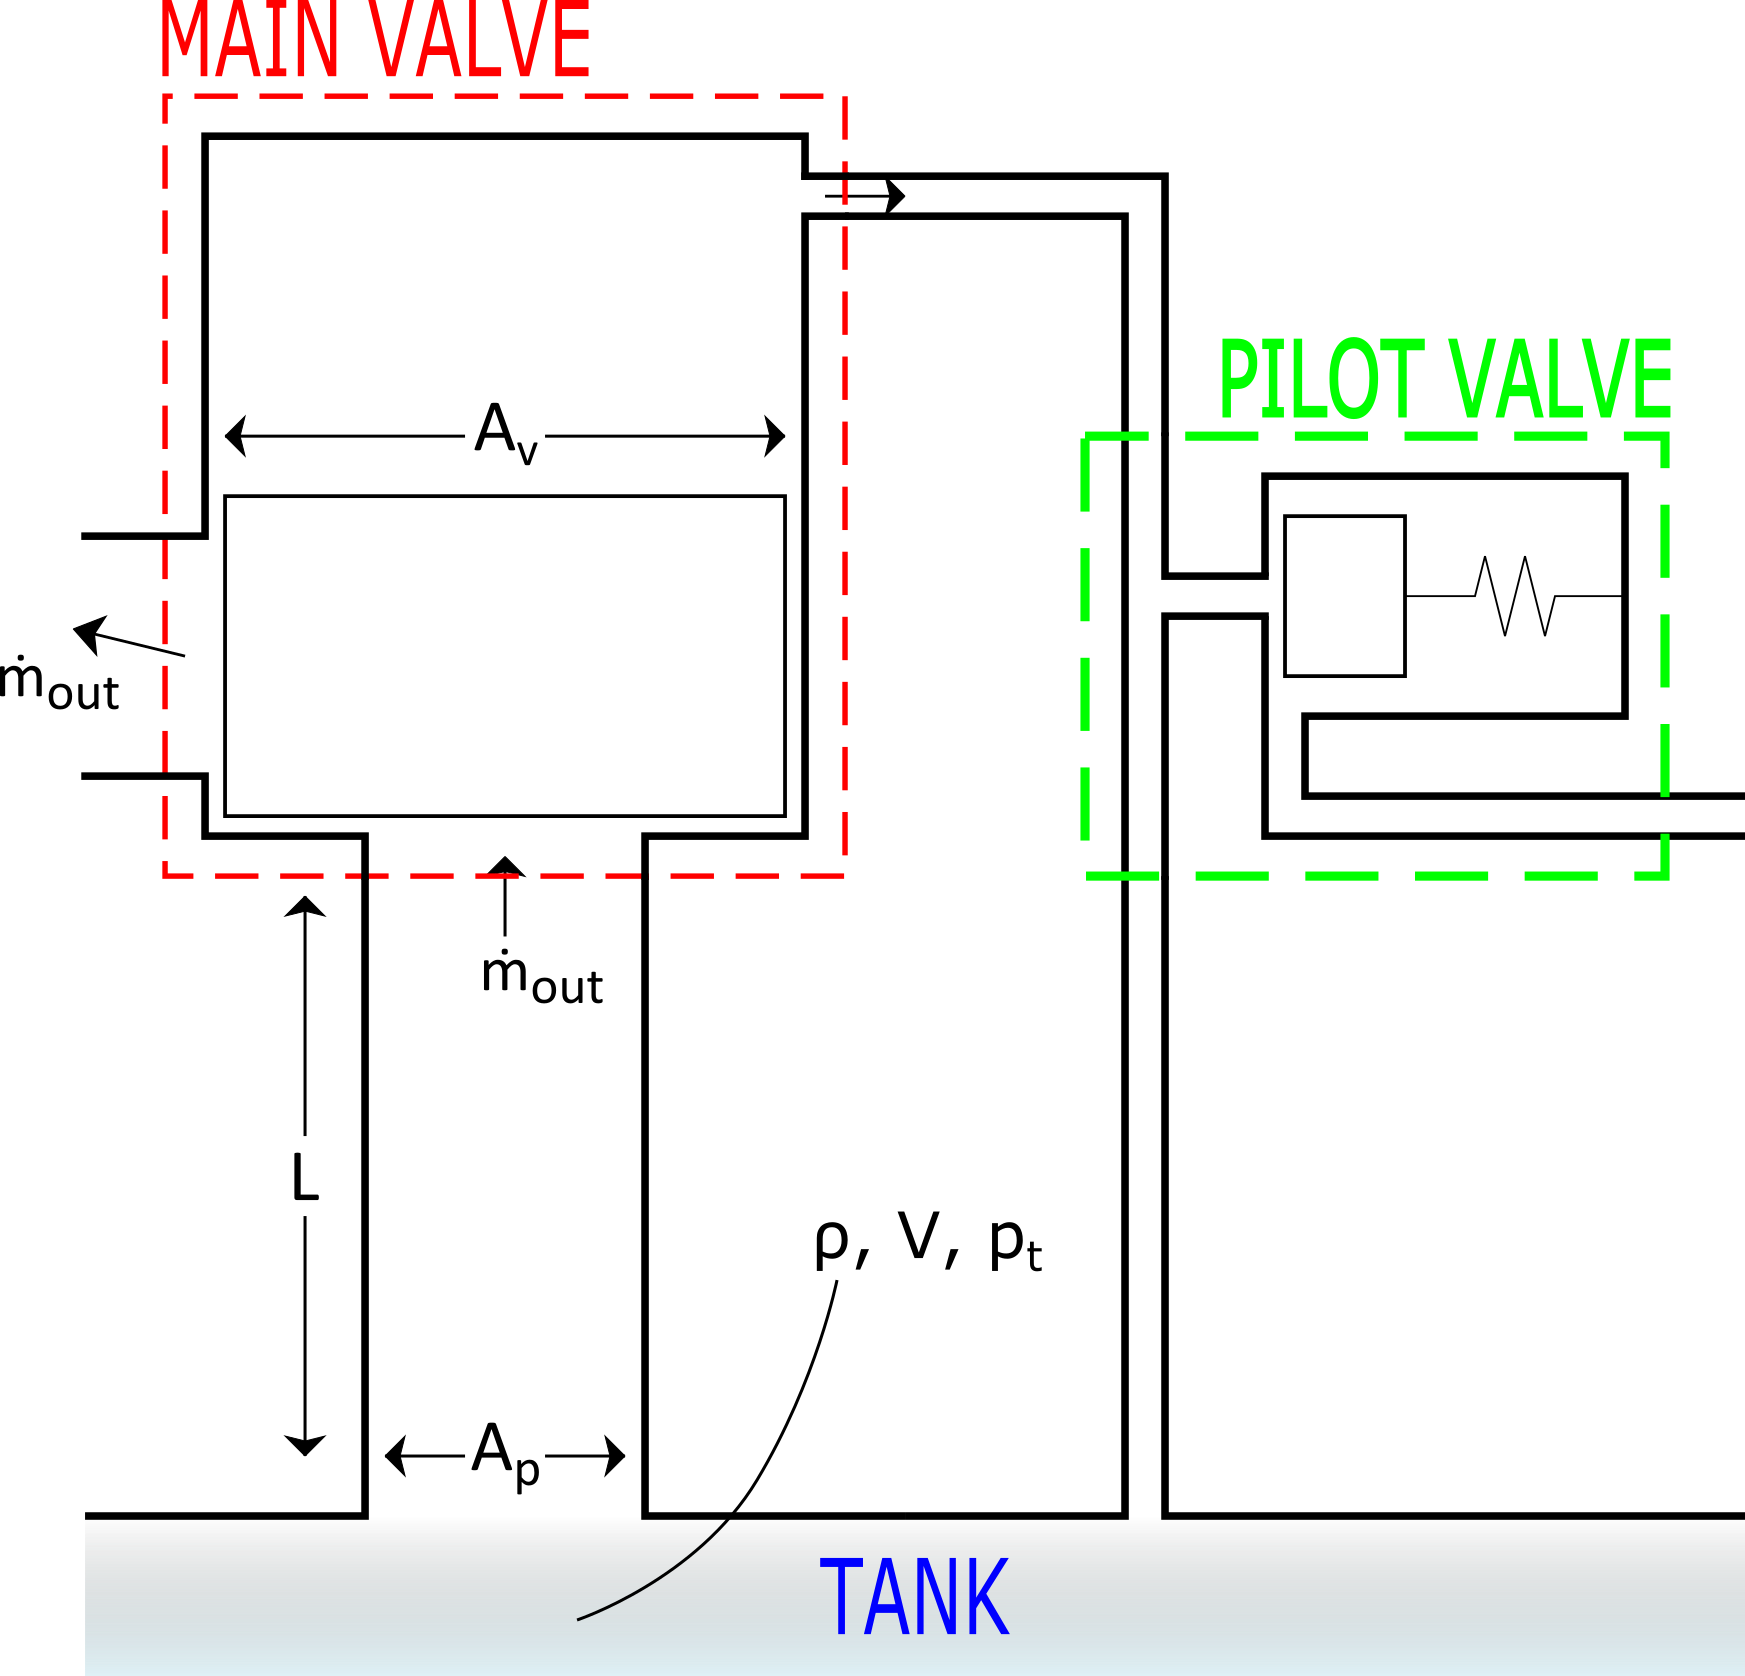
\includegraphics[width=\textwidth]{Diagrams/Diagram.png}
    \caption{Complete valve}
    \label{fig: DiagramComp}
    \end{subfigure}
    \hfill
    % Separate valve figures
    \begin{minipage}{0.3\textwidth}
        % MAIN DIAGRAM
        \begin{subfigure}{\textwidth}
        \centering
        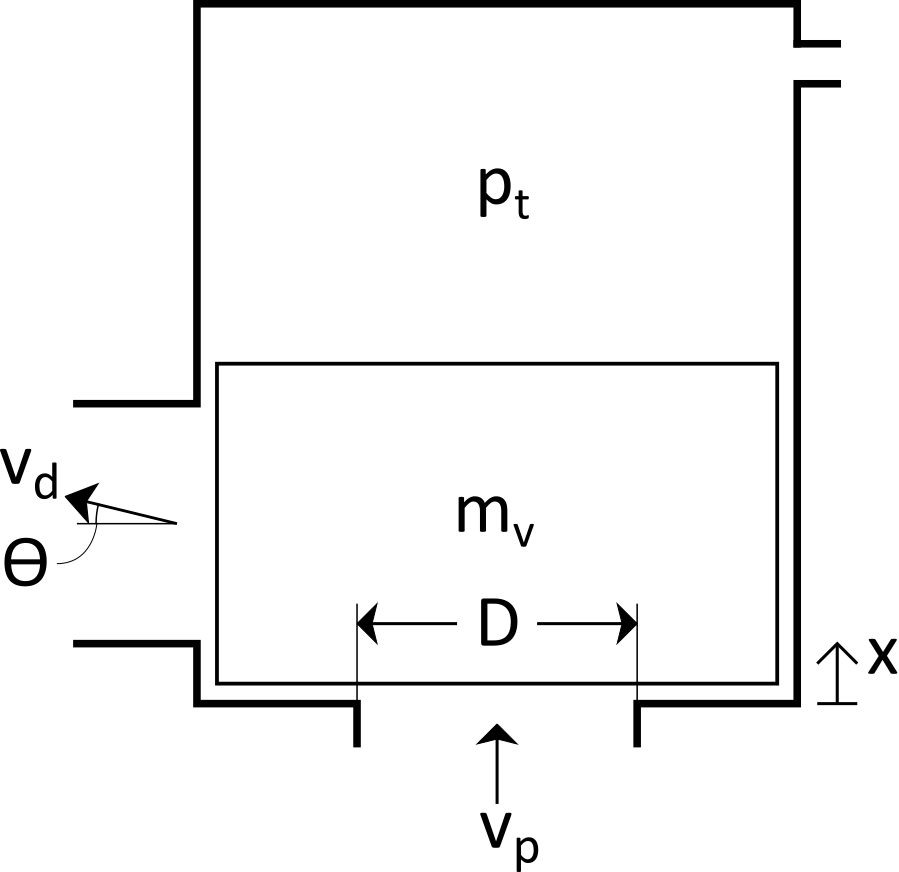
\includegraphics[width=\textwidth]{Diagrams/Diagram-Main.png}
        \caption{Main Valve}
        \label{fig: DiagramMain}
        \end{subfigure}
        % PILOT DIAGRAM
        \begin{subfigure}{\textwidth}
        \centering
        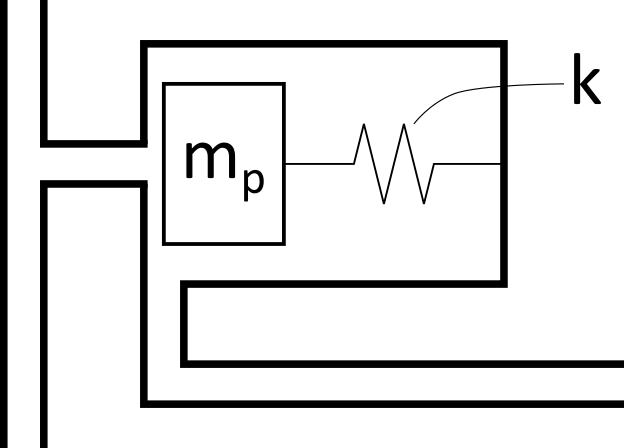
\includegraphics[width=\textwidth]{Diagrams/Diagram-Pilot.png}
        \caption{Pilot Valve}
        \label{fig: DiagramPilot}
        \end{subfigure}
    \end{minipage}
    % Figure caption and label
    \caption{Diagram of pilot-operated pressure relief valve}
    \label{fig: Diagram}
\end{figure}
%\end{figure}

Within the main valve, the fluid can be considered to act on the piston in three ways. The pressure above the piston, in the volume known as the dome, exerts a pressure force across the piston area, $A_v$. This dome pressure is assumed to be equal to the tank pressure. The jet of fluid from the inlet piping exerts a pressure and undergoes change of momentum due to the valve. For simplicity, the jet of fluid is assumed to act over an area equal to the piping cross-sectional area, $A_p$. The force exerted on the valve is equal to the momentum change exerted by the valve to cause the fluid to change flow direction. Combining all of these forces, the motion of the main valve piston can be described by
%\subsection{Valve closing}

\begin{equation} \label{eq: Newton}
    m_v \ddot{x} + c_v \dot{x} = - A_v p_t + A_p p_p + \dot{m}_{out} \left( v_p - v_d \sin(\theta) \right) \, .
\end{equation}

Here, $m_v$ is the valve piston mass, $c_v$ is the valve damping, $p_p$ is the pressure at the end of the pipe, and $\theta$ is the discharge angle. $v_p$ is the velocity of the fluid between the main valve and tank through the orifice or zero length pipe, which will now simply be referred to as the pipe velocity.

%\newpage
Clearly, the properties which depend on fluid dynamics must be expressed in terms of the piston position, $x$, and tank pressure, $p_t$. Firstly, the discharge velocity can be calculated by considering the conversion of static pressure into kinetic energy.

%\newpage
Hence, the discharge velocity is given by

\begin{equation} \label{eq: DisVel}
    v_d = C_d \sqrt{\frac{2 p_t}{\rho}} \, .
\end{equation}

Once the discharge velocity is known, the mass flow rate leaving the tank can be calculated as $\dot{m}_{out} = \rho A_d v_d$, where $A_d$ is the area through which the fluid is discharged. This area is the cylinder formed between the pipe outlet and the main valve piston. Therefore, the mass flow rate can be expressed as

\begin{equation*}
    \dot{m}_{out} =
%    \rho \left( \frac{\pi D^2}{4} \right) v_p =
    \rho \,\, \pi D x \cos(\theta) \,\, v_d \, ,
\end{equation*}

where $D$ is the diameter of the pipe and $\rho$ is the fluid density. The discharge velocity, $v_d$, is given by \cref{eq: DisVel}. The pipe velocity, $v_p$, can be calculated by equating the mass flow through the pipe with that being discharged from the valve. Hence,
%Hence, the velocity flow through the pipe, $v_p$, is given by

\begin{equation*}
    v_p = C_d \frac{4 x \cos(\theta)}{D} \sqrt{\frac{2 p_t}{\rho}} \, .
\end{equation*}

Finally, the static pressure acting on the bottom of the piston must be calculated. This static pressure will be equal to the tank pressure, with some pressure being converted into kinetic energy because of the fluid flow. Applying Bernoulli's equation, neglecting the change in gravitational potential, expresses $p_p$ as

\begin{equation*}
    p_p = p_t - \frac{1}{2} \rho v_p ^2 =
    %p_t - \frac{1}{2} \rho \left( C_d \frac{4 x \cos(\theta)}{D} \sqrt{\frac{2 p_t}{\rho}} \right)^2 =
    p_t \left( 1 - C_d \,^2 \left( \frac{4 x \cos(\theta)}{D} \right)^2 \right) \, .
\end{equation*}

All of the fluid properties calculated can be substituted into the piston equation of motion, given by~\cref{eq: Newton}. This yields the final equation of motion describing the piston motion,

\begin{equation} \label{eq: DiffEqValve}
    m_v \ddot{x} + c_v \dot{x} = p_t \left(
    C_d \,^2 \left( 4 \pi \cos^2(\theta) x^2
    - 2 \pi D \sin(\theta) \cos(\theta) x \right)
    - \left( A_v - \frac{\pi D^2}{4} \right)
    \right) \, .
\end{equation}

Finally, the equation for the pressure within the tank must be found. Obviously, any fluid flowing into the tank will increase the pressure. Conversely, the fluid leaving the tank through the PRV will decrease the pressure. Previous work identifies the relationship between tank pressure and mass flow rates~\cite{Hos2015DynamicModelling}. This allows the pressure to be expressed by

\begin{equation} \label{eq: DiffEqPres}
    \dot{p}_t = \frac{a^2}{V} \left( \dot{m}_{in} - \dot{m}_{out} \right) \, ,
\end{equation}

where $a$ is the sonic velocity, $V$ is the volume of the tank, and $\dot{m}_{in}$ and $\dot{m}_{out}$ are the mass flow rates in and out of the tank respectively.

Hence, the system of differential equations representing the main valve closing is given by \cref{eq: DiffEqValve,,eq: DiffEqPres}. These form a nonlinear system of differential equations, which will be now be analysed.

\subsection{Equilibrium}

% Calculating the equilibrium of the system gives a quadratic in $x$, which when solved gives

% \begin{equation*}
%     x_+ = \frac{D}{4} \tan(\theta) + \sqrt{
%     \frac{\frac{\pi D^2}{4} C_d \,^2 \sin^2(\theta) + A_v - \frac{\pi D^2}{4}}{4 \pi C_d \,^2 \cos^2(\theta)}
%     }
% \end{equation*}

% It can be shown that the negative root, $x_- \leq 0$, and as such can be ignored. %$x_- = 0 \implies \theta = \frac{\pi}{2}$ and hence is a non-meaningful physical solution.

%\subsection{No Discharge Angle}

Firstly, the steady state of \cref{eq: DiffEqValve,,eq: DiffEqPres} must be calculated. To simplify the expression of the steady state, the discharge angle $\theta$ will be assumed to be zero. The steady state of the system is calculated by equating the derivatives to zero. This gives equilibrium as

\begin{equation*}
    x_0 = \frac{1}{C_d} \sqrt{\frac{A_v - \frac{\pi D^2}{4}}{4 \pi}}
    \, , \quad
    p_0 = \frac{\dot{m}_{in} \,^2}{2 \frac{\pi D^2}{4} \left( A_v - \frac{\pi D^2}{4} \right)} \, .
\end{equation*}

% This gives the equilibrium pressure as

% \begin{equation*}
%     p_t = \frac{\dot{m}_{in} \,^2}{2 \frac{\pi D^2}{4} \left( A_v - \frac{\pi D^2}{4} \right)}
% \end{equation*}

\subsection{Non-dimensionalisation}

Before further analysis is performed, it is useful to express the system in terms of dimensionless variables. The dimensionless variables needed are displacement, pressure and time; which can be expressed in terms of reference parameters. For displacement and pressure, the steady state values are used as reference variables. The non-dimensional parameter used are

\begin{equation*}
    \tilde{x} = \frac{x}{x_{0}} \, ; \qquad
    \tilde{p} = \frac{p_t}{p_{0}} \, ; \qquad 
    \tilde{t} = t \cdot \frac{c_v}{m_v} \, .
\end{equation*}

%  The reference dimension for the time variable is given by

% \begin{equation*}
% %    x_{ref} = \frac{1}{C_d} \sqrt{\frac{A_v - \frac{\pi D^2}{4}}{4\pi}} ; \qquad
% %    p_{ref} = \frac{1}{2} \frac{\dot{m}_{in}\,^2}{\rho \left( \frac{\pi D^2}{4} \right) \left( A_v - \frac{\pi D^2}{4} \right)} \, ; \qquad
%     t_{ref} = \frac{m_v}{c_v} \, .
% \end{equation*}

By calculating the derivatives for the non-dimensional variables, \cref{eq: DiffEqValve,,eq: DiffEqPres} can be expressed as dimensionless equations. It can be shown that applying these variable transformation leads to the system of equations,

\begin{equation} \label{eq: Non-DimODE}
\begin{split}
    \tilde{x}'' + \tilde{x}' &= \alpha \, \tilde{p} \, \left( \tilde{x}^2 - 1 \right) \, ,\\
    \tilde{p}' &= \beta \left( 1 - \tilde{x} \sqrt{\tilde{p}} \right) \, .
\end{split}
\end{equation}

Here, the dimensionless constants $\alpha$ and $\beta$ are given by

\begin{equation*}
    \alpha = %\frac{4 \pi C_d \,^2}{m_v} x_{ref} p_{ref} t_{ref} =
    \frac{\sqrt{\pi} \, C_d \, m_v \, \dot{m}_{in}\,^2}{\rho \, c_v\,^2 \left( \frac{\pi D^2}{4} \right) \sqrt{A_v - \frac{\pi D^2}{4}} } \, , %\\
    \qquad
    \beta = %\frac{a^2}{V} \frac{t_ref}{p_ref} \dot{m}_{in} =
    \frac{ 2 \, \rho \, a^2 \, m_v \left( \frac{\pi D^2}{4} \right) \left( A_v - \frac{\pi D^2}{4} \right) }{ c_v \, V \, \dot{m}_{in} } \, .
%    \\ \mu = \frac{c_v}{m_v} t_{ref}
\end{equation*}

\subsection{Parameter Values}

Typical values for the parameters are given in the table below. Some from \cite{Hos2016DynamicService}.

\begin{table}[ht]
    \centering
    \begin{tabular}{c|c|c|c}
        Symbol & Description & Value & Units \\ \hline \hline
        $m_v$ & Main valve piston mass & ? & \si{kg} \\ \hline % NEED TO GET
        $c_v$ & Main valve damping coefficient & ? & \si{kg.s^{-1}} \\ \hline % NEED TO GET
        $C_d$ & Fluid discharge coefficient & ? & - \\ \hline % Alans paper uses 0.32
        $D$ & Inlet pipe diameter & 0.0266 & \si{m} \\ \hline % Valve 1E2 from \cite{Hos2016DynamicService}
        $A_p$ & Inlet pipe area & ? & \si{m^2} \\ \hline
        $A_v$ & Main valve piston area & ? & \si{m^2} \\ \hline
        $\dot{m}_{in}$ & Mass flow rate into tank & 0-3.8 & \si{kg.s^{-1}} \\ \hline % Valve 1E2 from \cite{Hos2016DynamicService}
        $\rho$ & Density of fluid & ? & \si{kg.m^{-3}} \\ \hline % Valve 1E2 from \cite{Hos2016DynamicService}
        $a$ & Sonic velocity & 890 & \si{m.s^{-1}} \\ \hline % Valve 1E2 from \cite{Hos2016DynamicService}
        $V$ & Tank volume & 10.6 & \si{m^3} \\ \hline % Valve 1E2 from \cite{Hos2016DynamicService}
        $r$ & Coefficient of restitution & 0.9 & - \\ \hline \hline % r = 0.8 in \cite{Hos2016DynamicService}
        $\alpha$ & First Dimensionless Parameter & ? & - \\ \hline
        $\beta$ & Second Dimensionless Parameter & ? & - \\
    \end{tabular}
    \caption{Caption}
    \label{tab:my_label}
\end{table}

\subsection{Stability Analysis}

% Firstly, the second order differential equation must be re-written as two first order differential equations. The system of three equations is

% \begin{equation*}
% \begin{split}
%     \tilde{x}' &= y \\
%     \tilde{y}' &= - y + \alpha \tilde{p} \left( \tilde{x}^2 - 1 \right) \\
%     \tilde{p}' &= \beta \left( 1 - \tilde{x} \sqrt{\tilde{p}} \right)
% \end{split}
% \end{equation*}

% Hence, the Jacobian of the system can be written as

% \begin{equation*}
%     \mathbf{J} =
%     \begin{pmatrix}
%     0 & 1 & 0 \\
%     2 \alpha \tilde{p} \tilde{x} & -1 & \alpha \left( \tilde{x}^2 - 1 \right) \\
%     - \beta \sqrt{\tilde{p}} & 0 & - \frac{1}{2} \frac{\beta \tilde{x} }{\sqrt{\tilde{p}}}
%     \end{pmatrix}
% \end{equation*}

% Evaluated at the positive equilibrium, $\left( \tilde{x},\tilde{y},\tilde{p} \right) = \left( 1,0,1 \right)$, the Jacobian simplifies to

% \begin{equation*}
%     \mathbf{J} =
%     \begin{pmatrix}
%     0 & 1 & 0 \\
%     2 \alpha & -1 & 0 \\
%     - \beta & 0 & - \frac{1}{2} \beta
%     \end{pmatrix}
% \end{equation*}

As the equilibrium for the system of differential equations has been calculated and transformed into a non-dimensional form, local stability analysis can be performed. The system is linearised around the equilibrium by calculating the Jacobian for the system described by \cref{eq: Non-DimODE}. This involves re-writing the second-order differential equation as two first-order differential equations. The local stability of the equilibrium is determined by the eigenvalues of the Jacobian matrix. These eigenvalues are given by

\begin{equation*}
\lambda_1 = - \frac{1}{2} \beta \, , \quad
\lambda_2 = - \frac{1}{2} - \sqrt{2 \alpha + \frac{1}{4}} \, , \quad \lambda_3 = - \frac{1}{2} + \sqrt{2 \alpha + \frac{1}{4}} \, .
\end{equation*}

From the definition of the two non-dimensional parameters, $\alpha$ and $\beta$, it can be seen than both must be positive constants. Because $\alpha > 0$ and $\beta > 0$, exactly one eigenvalue is positive so the equilibrium is a saddle. Because of the positive eigenvalue, the equilibrium is unstable. This suggests the main valve will not remain open, which may explain why the main valve closes. However, a potential concern of this model is, if the main valve lift rises above the open position equilibrium, then it will continually increase to infinity.

The corresponding eigenvalues are given by

\begin{equation*}
    v_1 = \begin{pmatrix}
    0 \\ 0 \\ 1
    \end{pmatrix} \qquad
    v_2 = \begin{pmatrix}
    \frac{1}{2\beta} \left( 1 + \sqrt{8\alpha+1} \right) - \frac{1}{2} \\ \frac{1}{4\beta} \left( 1 + \sqrt{8\alpha+1} \right) \left( \beta - 2 \right) - \frac{2\alpha}{\beta} \\ 1
    \end{pmatrix} \qquad
    v_3 = \begin{pmatrix}
    \frac{1}{2\beta} \left( 1 - \sqrt{8\alpha+1} \right) - \frac{1}{2} \\ \frac{1}{4\beta} \left( 1 - \sqrt{8\alpha+1} \right) \left( \beta - 2 \right) - \frac{2\alpha}{\beta} \\ 1
    \end{pmatrix}
\end{equation*}

\subsection{Simulations}

For $\alpha = 0.1$ and $\beta = 1$, the simulation results are shown below

\begin{figure}[!ht]
    \centering
    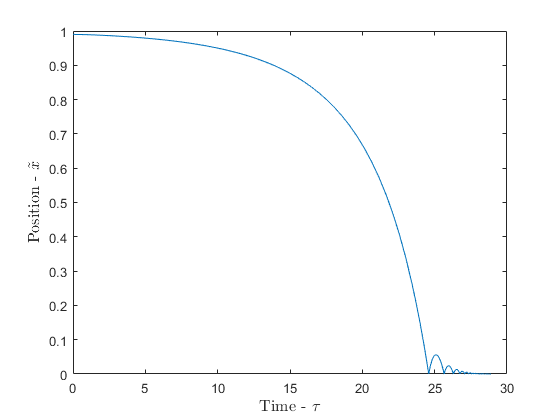
\includegraphics[width=0.6\textwidth]{Figures/Example/PositionTimeTrajectory.png}
    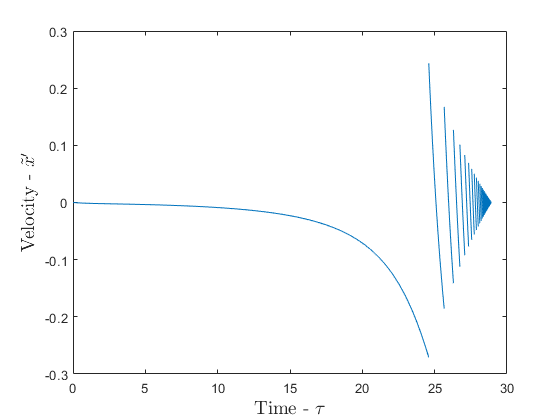
\includegraphics[width=0.49\textwidth]{Figures/Example/VelocityTimeTrajectory.png}
    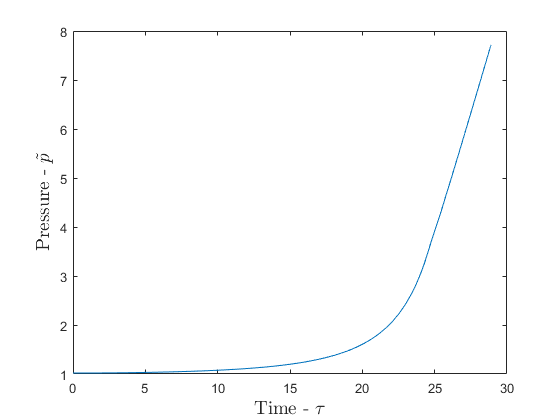
\includegraphics[width=0.49\textwidth]{Figures/Example/PressureTimeTrajectory.png}
    \caption{Caption}
    \label{fig:TimeTrajec}
\end{figure}

\begin{figure}[!ht]
    \centering
    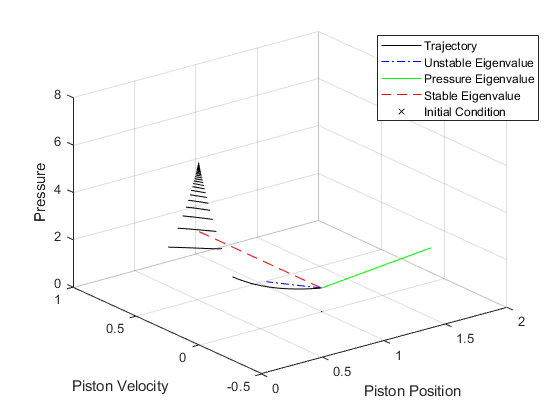
\includegraphics[width=0.49\textwidth]{Figures/Example/PhasePotrait3D.png}
    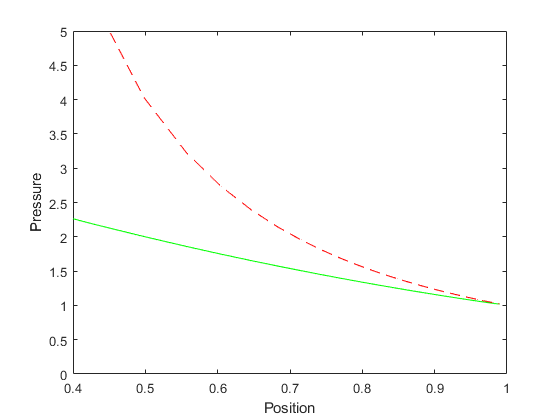
\includegraphics[width=0.49\textwidth]{Figures/Example/PressurePositionPhasePotrait2D.png}
    \caption{Caption}
    \label{fig:ExamplePhase}
\end{figure}

\begin{figure}[!ht]
    \centering
    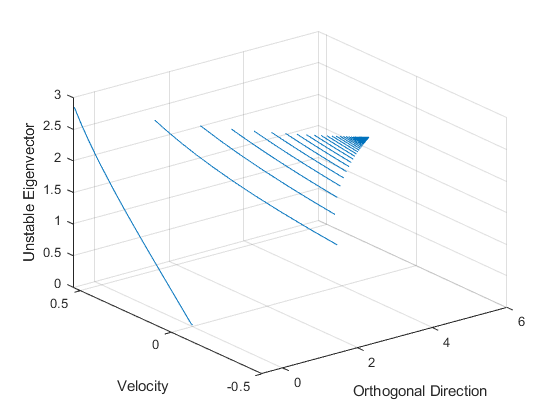
\includegraphics[width=0.7\textwidth]{Figures/Example/EigenvectorPhasePotrait3D.png}
    \caption{Caption}
    \label{fig:EigPhase}
\end{figure}

\begin{figure}[!ht]
    \centering
    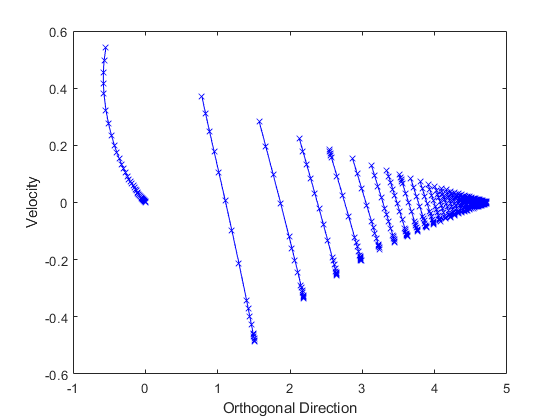
\includegraphics[width=0.49\textwidth]{Figures/Example/PhasePotrait2D.png}
    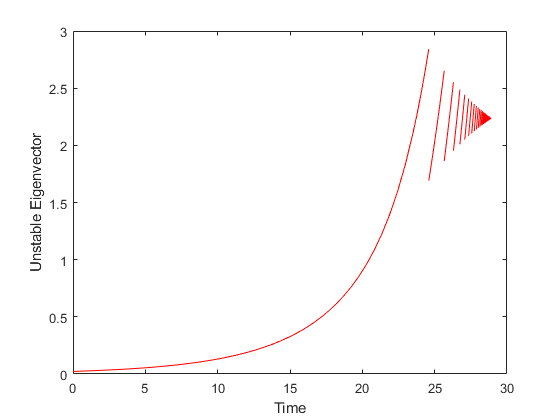
\includegraphics[width=0.49\textwidth]{Figures/Example/UnstableEigenvectorTrajectory.png}
    \caption{Caption}
    \label{fig:EigenvectorPhase}
\end{figure}

\newpage
\subsection{Low flow rates}

For low flow rates, $\dot{m}_{in} \rightarrow 0$, meaning that $\alpha \rightarrow 0$ and $\beta \rightarrow \infty$. Considering only the limit as $\alpha \rightarrow 0$, the eigenvalues and eigenvectors are

\begin{equation*}
\begin{split}
    % eigenvalues
    \lambda_1 = - \frac{1}{2}\beta \, , \quad
    \lambda_2 = -1 \, , \quad
    \lambda_3 = 0 \\
    % eigenvectors
    v_1 = \begin{pmatrix}
    0 \\ 0 \\ 1
    \end{pmatrix} \qquad
    v_2 = \begin{pmatrix}
    \frac{2 - \beta}{2\beta} \\ \frac{\beta - 2}{2\beta} \\ 1
    \end{pmatrix} \qquad
    v_3 = \begin{pmatrix}
    - \frac{1}{2} \\ 0 \\ 1
    \end{pmatrix}
\end{split}
\end{equation*}

The dynamics approach the equation

\begin{equation*}
    1 - x \sqrt{p} = 0 \, .
\end{equation*}

Simulation results support this. 

\begin{figure}[ht]
    \centering
    \begin{subfigure}{0.49\textwidth}
    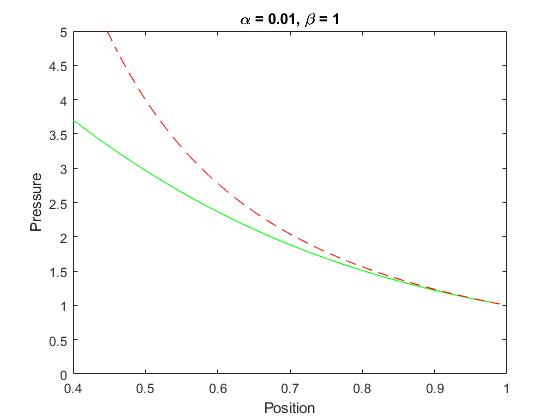
\includegraphics[width=\textwidth]{Figures/LowFlow/b=1.png}
    \caption{$\alpha = 0.01, \, \beta = 1$}
%    \label{fig:1}
    \end{subfigure}
    \begin{subfigure}{0.49\textwidth}
    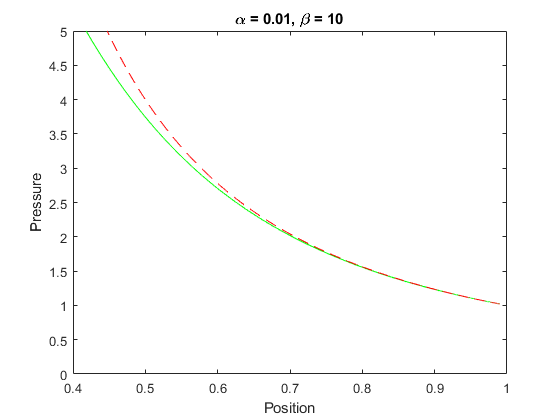
\includegraphics[width=\textwidth]{Figures/LowFlow/b=10.png}
    \caption{$\alpha = 0.01, \, \beta = 10$}
%    \label{fig:2}
    \end{subfigure}
%    \label{3}
%    \caption{}
\end{figure}

The phase portrait in Position-Pressure space can be seen below

\begin{figure}[ht]
    \centering
    \begin{subfigure}{0.49\textwidth}
    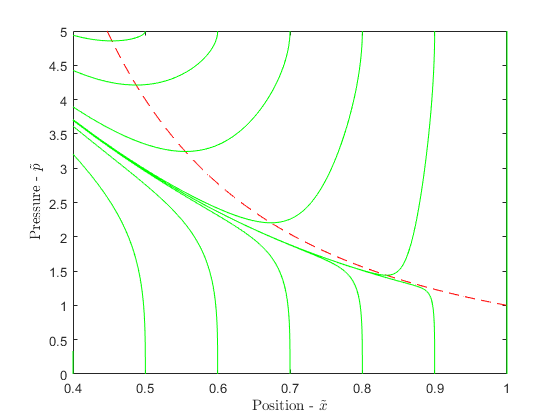
\includegraphics[width=\textwidth]{Figures/LowFlow/PhasePortrait-b=1.png}
    \caption{$\alpha = 0.01, \, \beta = 1$}
%    \label{fig:1}
    \end{subfigure}
    \begin{subfigure}{0.49\textwidth}
    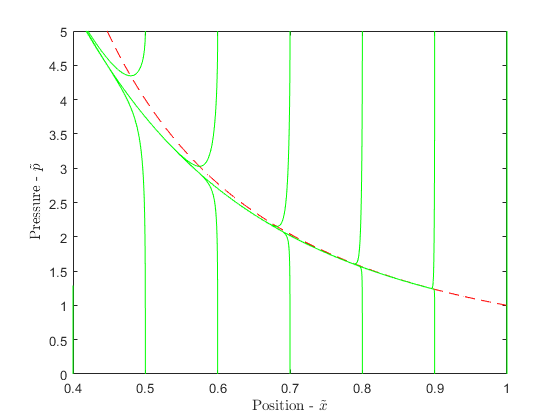
\includegraphics[width=\textwidth]{Figures/LowFlow/PhasePortrait-b=10.png}
    \caption{$\alpha = 0.01, \, \beta = 10$}
%    \label{fig:2}
    \end{subfigure}
%    \label{3}
%    \caption{}
\end{figure}